% Inference on Ceilings: Chandelier Debiasing for Optimal Policy Value with Continuous Treatments under Preference Data
% Inference on the peak ("ceiling") of a value curve over a continuous treatment, learned from pairwise preferences.
\documentclass[tikz,border=0pt]{standalone}
% Shared look for the TikZ publication thumbnails.
% Canvas: 16cm x 10cm (16:10, matching the 640x400 WebP output), white, site palette.
% Labels are large (\lbl) because thumbnails are shown about 200px wide.
\usepackage[T1]{fontenc}
\usepackage{helvet}
\renewcommand{\familydefault}{\sfdefault}
\usepackage{amsmath,amssymb}
\usepackage{fontawesome5}
\usetikzlibrary{arrows.meta,calc,positioning,shapes.geometric,shapes.callouts,decorations.pathmorphing,shadows}

\definecolor{ink}{HTML}{2B2D42}
\definecolor{accent}{HTML}{B509AC}
\definecolor{teal}{HTML}{1E9BC0}
\definecolor{violet}{HTML}{6C5CE7}
\definecolor{orange}{HTML}{F28C28}
\definecolor{sun}{HTML}{F2C14E}
\definecolor{leaf}{HTML}{2CA58D}
\definecolor{alert}{HTML}{E5484D}
\definecolor{mist}{HTML}{EEF0F5}

\tikzset{
  every picture/.append style={line cap=round, line join=round},
  card/.style={rounded corners=10pt, draw=#1!75!black, line width=1.4pt, fill=#1!12},
  arrow/.style={-{Stealth[length=10pt,width=9pt]}, line width=2.2pt, draw=#1},
  soft shadow/.style={drop shadow={shadow xshift=0pt, shadow yshift=-3pt, opacity=0.18, fill=ink}},
  badge/.style={circle, fill=#1!14, draw=#1, line width=2pt, minimum size=2.3cm, text=#1},
}
\newcommand{\thumbcanvas}{\useasboundingbox[fill=white] (0,0) rectangle (16,10);}
\newcommand{\lbl}[1]{{\fontsize{20}{22}\selectfont\bfseries #1}}
\newcommand{\icon}[2][34]{{\fontsize{#1}{#1}\selectfont\faIcon{#2}}}
% Window chrome: dark editor panel with traffic-light dots. Args: x0, y0, x1, y1.
\newcommand{\editor}[4]{%
  \fill[ink, rounded corners=12pt, soft shadow] (#1,#2) rectangle (#3,#4);
  \foreach \c [count=\k] in {alert,sun,leaf} \fill[\c] ({#1+0.15+0.42*\k},{#4-0.42}) circle (0.13);
}

\begin{document}
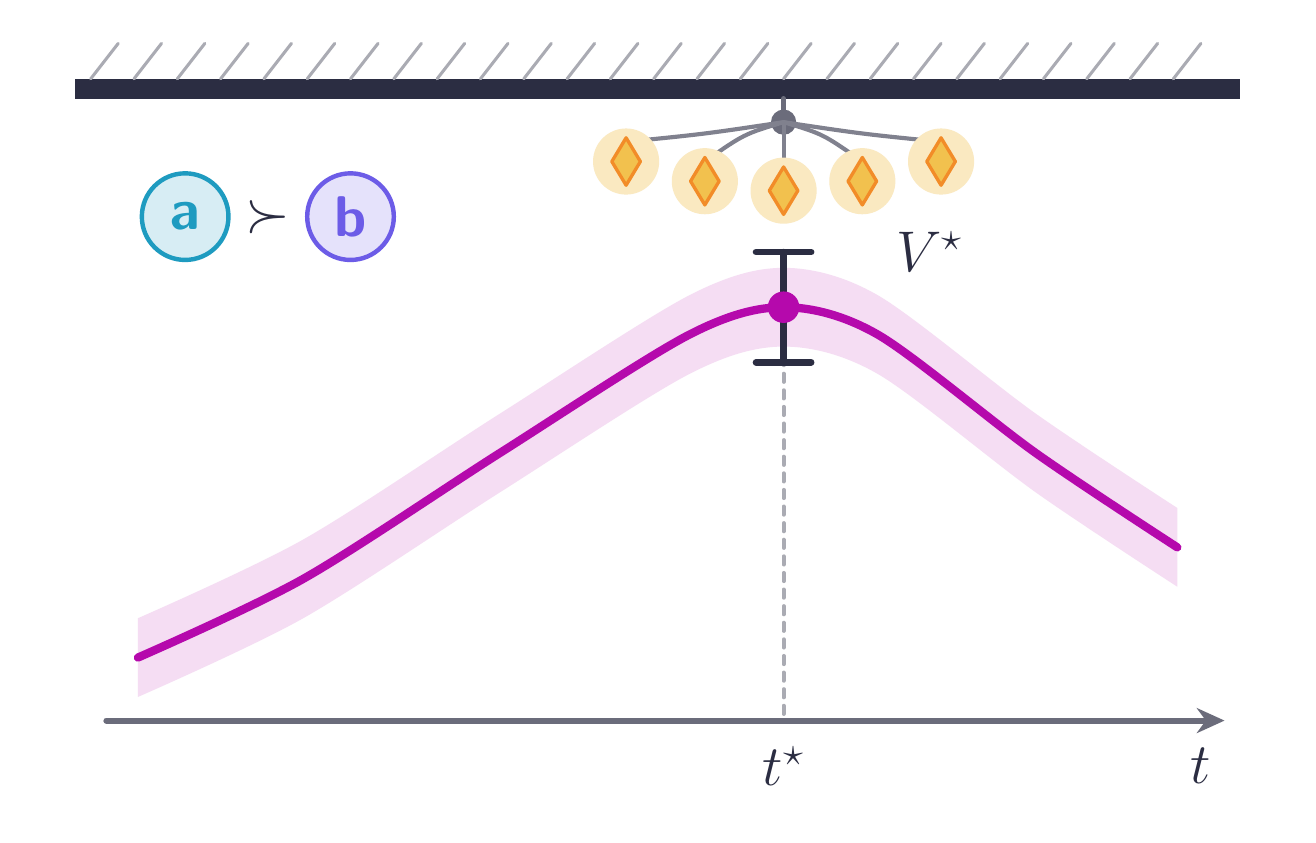
\begin{tikzpicture}
\thumbcanvas
% Ceiling.
\fill[ink] (0.6,9.1) rectangle (15.4,9.35);
\foreach \x in {0.8,1.35,...,15.1} \draw[ink!40, line width=1.1pt] (\x,9.35) -- ++(0.35,0.45);
% Schematic value curve over the treatment with an uncertainty band (no data).
\fill[accent!14]
  plot[smooth] coordinates {(1.4,2.5) (3.5,3.5) (6.0,5.1) (8.4,6.6) (9.6,6.95) (10.8,6.6) (12.8,5.1) (14.6,3.9)}
  -- plot[smooth] coordinates {(14.6,2.9) (12.8,4.1) (10.8,5.6) (9.6,5.95) (8.4,5.6) (6.0,4.1) (3.5,2.5) (1.4,1.5)}
  -- cycle;
\draw[accent, line width=3pt]
  plot[smooth] coordinates {(1.4,2.0) (3.5,3.0) (6.0,4.6) (8.4,6.1) (9.6,6.45) (10.8,6.1) (12.8,4.6) (14.6,3.4)};
\draw[arrow=ink!70] (1.0,1.2) -- (15.2,1.2);
\draw[dashed, ink!40, line width=1.4pt] (9.6,6.45) -- (9.6,1.2);
\node[text=ink] at (9.6,0.62) {\lbl{$t^\star$}};
\node[text=ink] at (14.9,0.62) {\lbl{$t$}};
% Inference on the optimal value: estimate with an interval.
\draw[ink, line width=2.4pt] (9.6,5.75) -- (9.6,7.15);
\draw[ink, line width=2.4pt] (9.25,5.75) -- (9.95,5.75) (9.25,7.15) -- (9.95,7.15);
\fill[accent] (9.6,6.45) circle (0.2);
\node[text=ink] at (11.45,7.15) {\lbl{$V^\star$}};
% The chandelier hangs from the ceiling right above the optimum.
\draw[ink!70, line width=1.8pt] (9.6,9.1) -- (9.6,8.85);
\fill[ink!70] (9.6,8.8) circle (0.16);
\foreach \dx/\dy in {-2.0/0.25,-1.0/0.5,0/0.62,1.0/0.5,2.0/0.25} {
  \draw[ink!60, line width=1.5pt] (9.6,8.8) .. controls ({9.6+0.5*\dx},8.65) .. ({9.6+\dx},{8.8-\dy});
  \fill[sun!35] ({9.6+\dx},{8.8-\dy-0.25}) circle (0.42);
  \node[diamond, fill=sun, draw=orange, line width=1.2pt, inner sep=0pt, minimum width=0.38cm, minimum height=0.62cm]
    at ({9.6+\dx},{8.8-\dy-0.25}) {};
}
% Preference data: pairwise comparisons.
\node[circle, fill=teal!18, draw=teal, line width=1.6pt, minimum size=1.1cm, text=teal] (a) at (2.0,7.6) {\lbl{a}};
\node[text=ink] at (3.05,7.6) {\lbl{$\succ$}};
\node[circle, fill=violet!18, draw=violet, line width=1.6pt, minimum size=1.1cm, text=violet] (b) at (4.1,7.6) {\lbl{b}};
\end{tikzpicture}
\end{document}
